\subsection*{\hypertarget{world}{Crear la Aventura}}
\addcontentsline{toc}{subsection}{Crear la Aventura}%
"Mundo ser muy simple. Mundo tener dos cosas: cosas que poder comer y cosas que no poder comer".\\
\indent -- Quina

\begin{center} 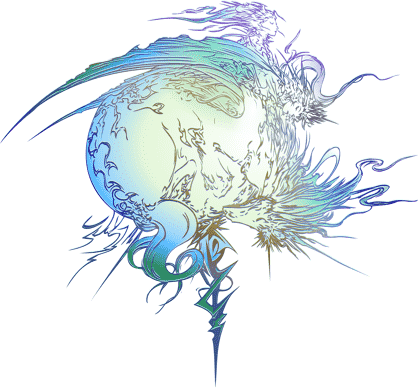
\includegraphics[width=1\columnwidth]{./art/images/ff13.png} \end{center}
\noindent
Crear un mundo es una de las partes más difíciles, pero también más gratificantes de ser DJ. Los jugadores son parte de tu mundo, donde interactúan con el entorno y lo cambian a través de sus acciones y decisiones. Por lo tanto, el mundo debería apreciar su curiosidad ofreciendo contenido interesante y permitiendo que sus decisiones sean significativas. Esta subsección ofrece algunas sugerencias sobre cómo crear un mundo interesante para tu partida.

\subsubsection*{Conflicto central}
La mayoría de las aventuras gira en torno a un conflicto central que el grupo tratará de resolver como objetivo de su aventura. Tradicionalmente, este conflicto implica múltiples fuerzas con intereses opuestos y los aventureros pueden formar parte de alguna de esas fuerzas. En consecuencia, también hay un lado opuesto, un enemigo en común o un antagonista que actúa en contra del grupo. Como DJ, asumes el papel de los personajes en distintos lados de este conflicto, por lo que debes considerar sus diferentes perspectivas.

\subsubsection*{Mapa}
Una buena forma de empezar a crear una aventura es establecer cómo se ve el mundo en un mapa. Empieza creando su medio ambiente (terreno, agua, bosques, montañas, desiertos, etc.). Después, coloca y marca lugares que podrían resultar interesantes para que los jugadores visiten, como ciudades, mazmorras o ruinas. A continuación, añade más detalles solo a los lugares que los jugadores probablemente visitarán al principio. Puedes hacerlo con el resto más adelante. Los jugadores podrían incluso obtener este mapa en algún momento del juego para que conozcan estos lugares que has creado.

\pagebreak

\subsubsection*{Personajes no jugadores}
Después de crear algunos lugares detallados, piensa quién podría vivir en estos lugares. Tú interpretarás a estos personajes no jugadores cuando interactúan con el grupo. Viven sus propias vidas independientemente de los jugadores y tienen sus propias personalidades, metas, habilidades y perspectivas de vida. En consecuencia, a menudo tienen conocimiento del mundo que los jugadores no poseen. Pueden ser aliados, neutrales o enemigos del grupo, dependiendo de las circunstancias. Para crear personajes no jugadores detallados, puedes utilizar la \hyperlink{char}{Guía de Creación de Personajes}, pero por lo general basta con anotar algunas cosas sobre ellos.

\subsubsection*{Magia}
Hay dos elementos de fantasía que son primordiales para el sistema de juego: la magia y los monstruos. Es importante establecer las fuentes de la magia y el papel que desempeña en tu mundo. En Final Fantasy, los cristales a menudo representan poderosas fuentes de magia y, por lo tanto, son el centro de muchos conflictos. A menudo también nos encontramos con seres mágicos llamados \hyperlink{summons}{Espers}, que representan las diferentes fuerzas de la naturaleza y están conectados a los cristales. Normalmente, los monstruos están conectados a las fuentes mágicas de alguna manera, por lo que pueden utilizar magia.

\subsubsection*{Tecnología}
El avance de la tecnología es otro aspecto importante a tener en cuenta para dar forma a tu mundo. Las diferentes tecnologías, como máquinas y armas, pueden complementar las fuerzas mágicas del mundo, pero también pueden estar en conflicto con ellas. Así, las sociedades de tu mundo pueden preferir la magia y la tecnología y confiar en ellas en distinta medida para sus vidas diarias. Durante su aventura, el grupo puede hacer uso de las tecnologías disponibles e incluso contribuir al desarrollo de las mismas.

\vspace{0.8cm}

\example{Crear la Aventura}
{
 El mundo que creamos consta de dos partes: Pulse y Cocoon. Pulse es un enorme planeta inexplorado con una vasta naturaleza que alberga a varios monstruos. En contraste, Cocoon es un pequeño planeta que flota por encima de Pulse y está habitado por una sociedad humana avanzada. Los ciudadanos Cocoon dependen de seres omniscientes para satisfacer sus necesidades como alimento y electricidad. Estos poderosos seres se llaman fal’Cie y pueden ejercer un control directo o indirecto sobre los seres humanos. Los fal’Cie de Cocoon están en conflicto contra los fal’Cie de Pulse y, en consecuencia, los humanos están condicionados a ser hostiles hacia Pulse. Nuestra aventura comienza en Cocoon, donde se descubrió un antiguo fal’Cie de Pulse hace algunos días. Como medida radical, el gobierno de Cocoon ordena la deportación de todos los humanos que hayan estado cerca del fal’Cie de Pulse. Pequeños grupos de ciudadanos rebeldes se unen para luchar contra esta denominada "Purga".
}

\pagebreak






